% 9 variables in here:
% h_1 = 10.0, h_2 = 12.0, h_3 = 7.0, ux_1 = 0.0, ux_2 = 0.0, ux_3 = 0.0, uy_1 = 0.0, uy_2 = 0.0, uy_3 = 0.0
\begin{figure}[h!]
\centering
  \subfloat[] {
    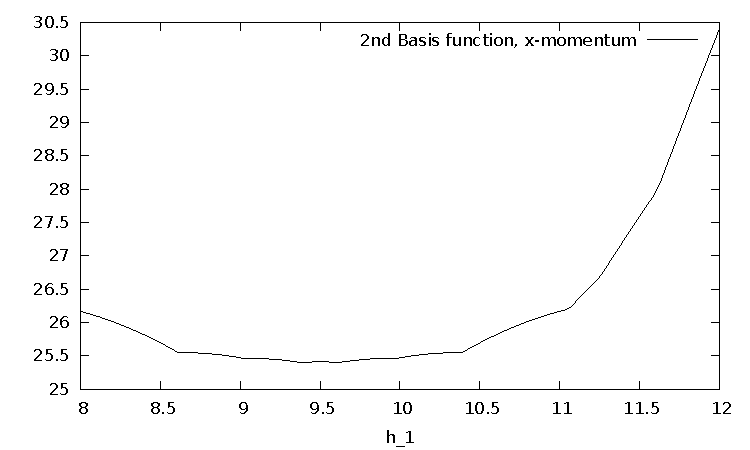
\includegraphics[scale=\zoomfactor]{{{magnitude_10_nonstd/y_12.0_7.0_0.0_0.0_0.0_0.0_0.0_0.0f02}}}
  }
\caption{}
\label{fig:magnitude_10_nonstd}
\end{figure}

%%% Local Variables:
%%% TeX-master: "../results.tex"
%%% End:
